% ANL Beamer template
\documentclass[aspectratio=169]{beamer}
\usepackage[english]{babel}
\usepackage[utf8]{inputenc}

% AMSLaTeX packages
\usepackage{amsthm}
\usepackage{amsmath}
\usepackage{amsfonts}
\usepackage[algoruled]{algorithm2e}

\usetheme{default}
\useoutertheme{default}
% we want to use images
\usepackage{graphicx}
\usepackage{movie15}
\usepackage{hyperref}

% table relates packages
\usepackage{booktabs}
\usepackage{multirow}
% pick a font
\usepackage{palatino}           
% \usepackage{times}
\usepackage{tikz}
\usetikzlibrary[positioning,arrows,decorations.pathmorphing,backgrounds,fit,calc]
% \AtBeginSection[]  % "Beamer, do the following at the start of every section"
% {
%   \begin{frame}<beamer> 
%     \frametitle{Outline} % make a frame titled "Outline"
%     \tableofcontents[currentsection]  % show TOC and highlight current section
%   \end{frame}                    
% }

% \AtBeginSubsection[]
% {
%   \begin{frame}
%     \frametitle{Outline}
%     \tableofcontents[currentsection,currentsubsection]
%   \end{frame}
% }

\AtBeginSection[]
{
   \begin{frame}
       \frametitle{Outline}
       \tableofcontents[currentsection]
   \end{frame}
}

\newcommand{\ebox}[1][1em]{\framebox[#1]{\phantom{M}}}

\setlength\arraycolsep{1.4pt}% some length

%gets rid of navigation symbols
\setbeamertemplate{navigation symbols}{}

%gets rid of bottom navigation bars
\setbeamertemplate{footline}[page number]{}
\setbeamertemplate{headline}{}


\usebackgroundtemplate{
\includegraphics[width=\paperwidth]{NormalANLBlue}}

% Define big arrow down
\newcommand{\xdownarrow}[1]{%
  {\left\downarrow\vbox to #1{}\right.\kern-\nulldelimiterspace}
}

\usepackage{xcolor,ulem}

% Title/author info
\title{ParMOO: A Python library for parallel multiobjective simulation optimization}
\author{Tyler Chang$^a$ and Stefan Wild$^a$}
\institute{$^a$Mathematics and Computer Science Division,\\
Argonne National Laboratory}
\date{FASTMath AHM 2022}

% Slides start here
\begin{document}

% Set the background graphics
\setbeamertemplate{footline}{}
{
\usebackgroundtemplate{
\includegraphics[width=\paperwidth]{TitleANLBlue}}
\frame{\titlepage}
}
\setbeamertemplate{footline}[page number]{}

%% FRAME: overview
%\begin{frame}
%  \frametitle{Outlines}
%  \tableofcontents
%\end{frame}

% ========================================
% main slides come here
% ========================================

\begin{frame}\frametitle{Multiobjective *Simulation* Optimization}
\begin{center}
\onslide<1>{
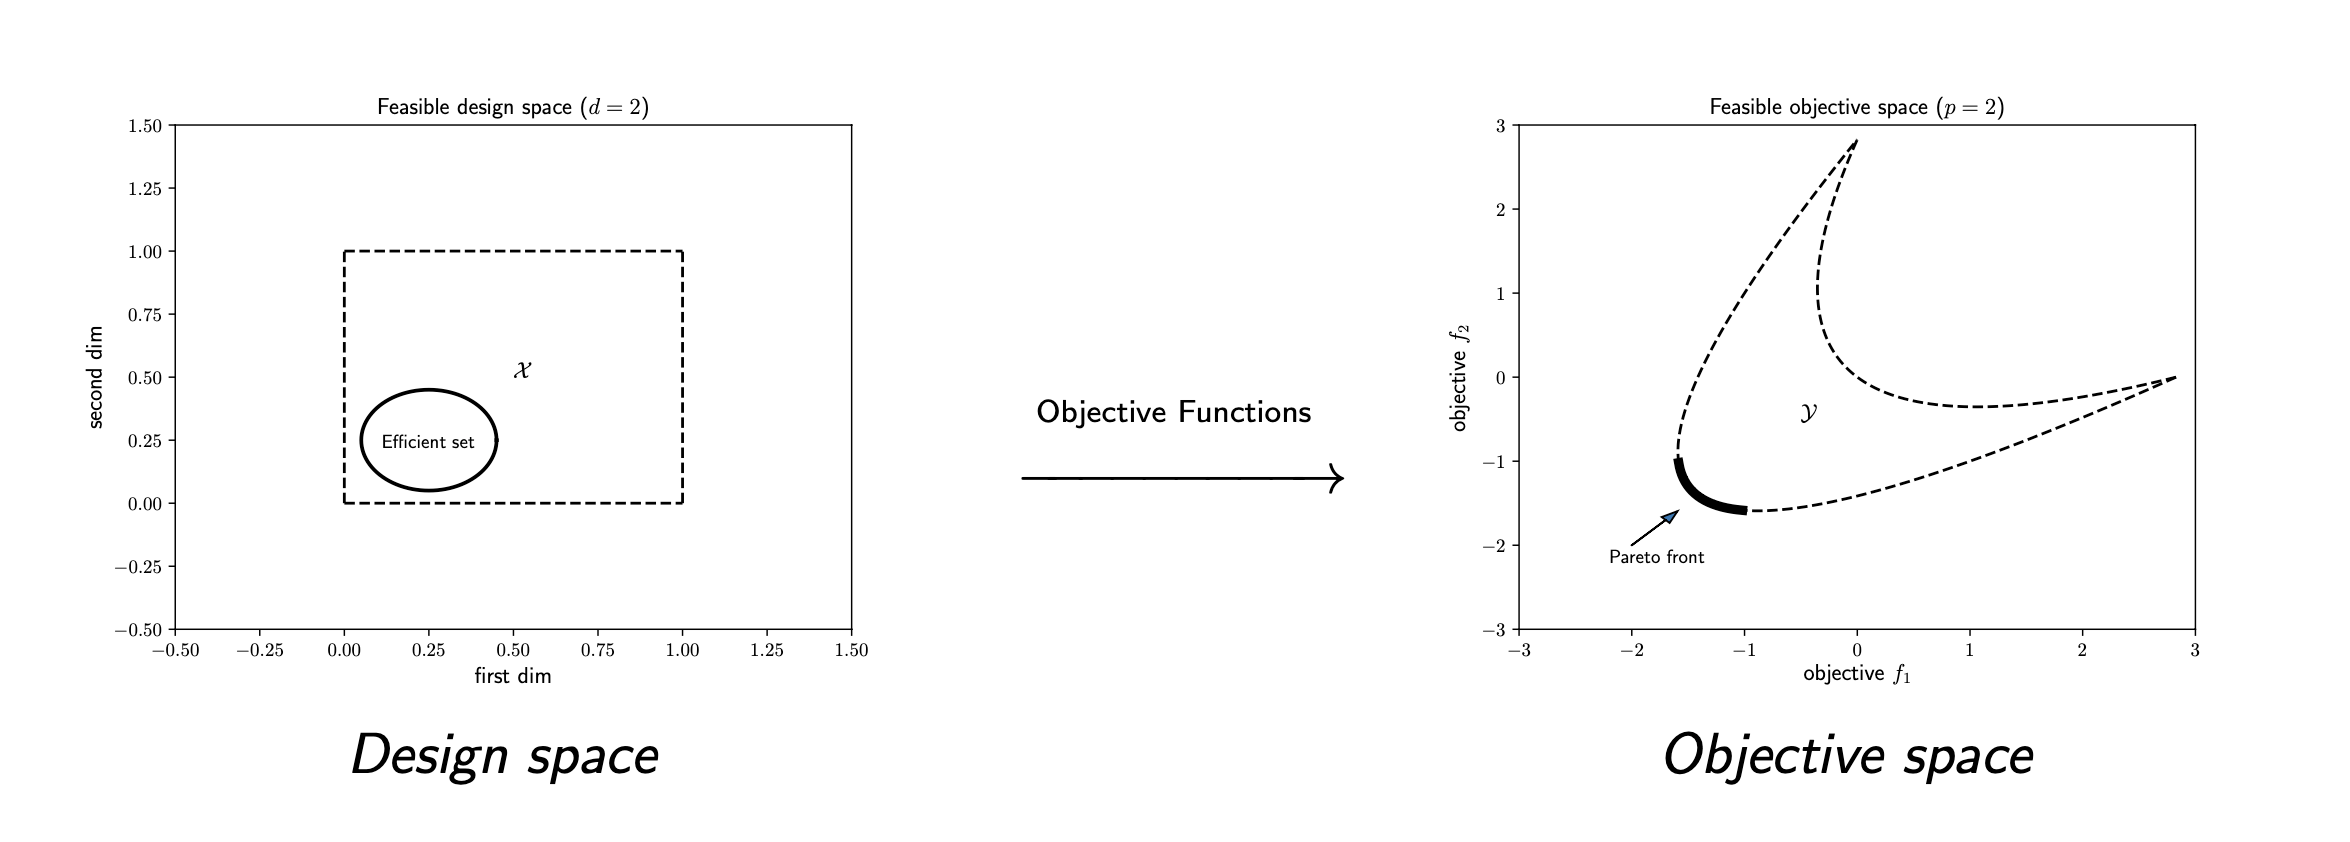
\includegraphics[height=2in]{des-obj-space.png}}

\vskip -2in

\onslide<2>{
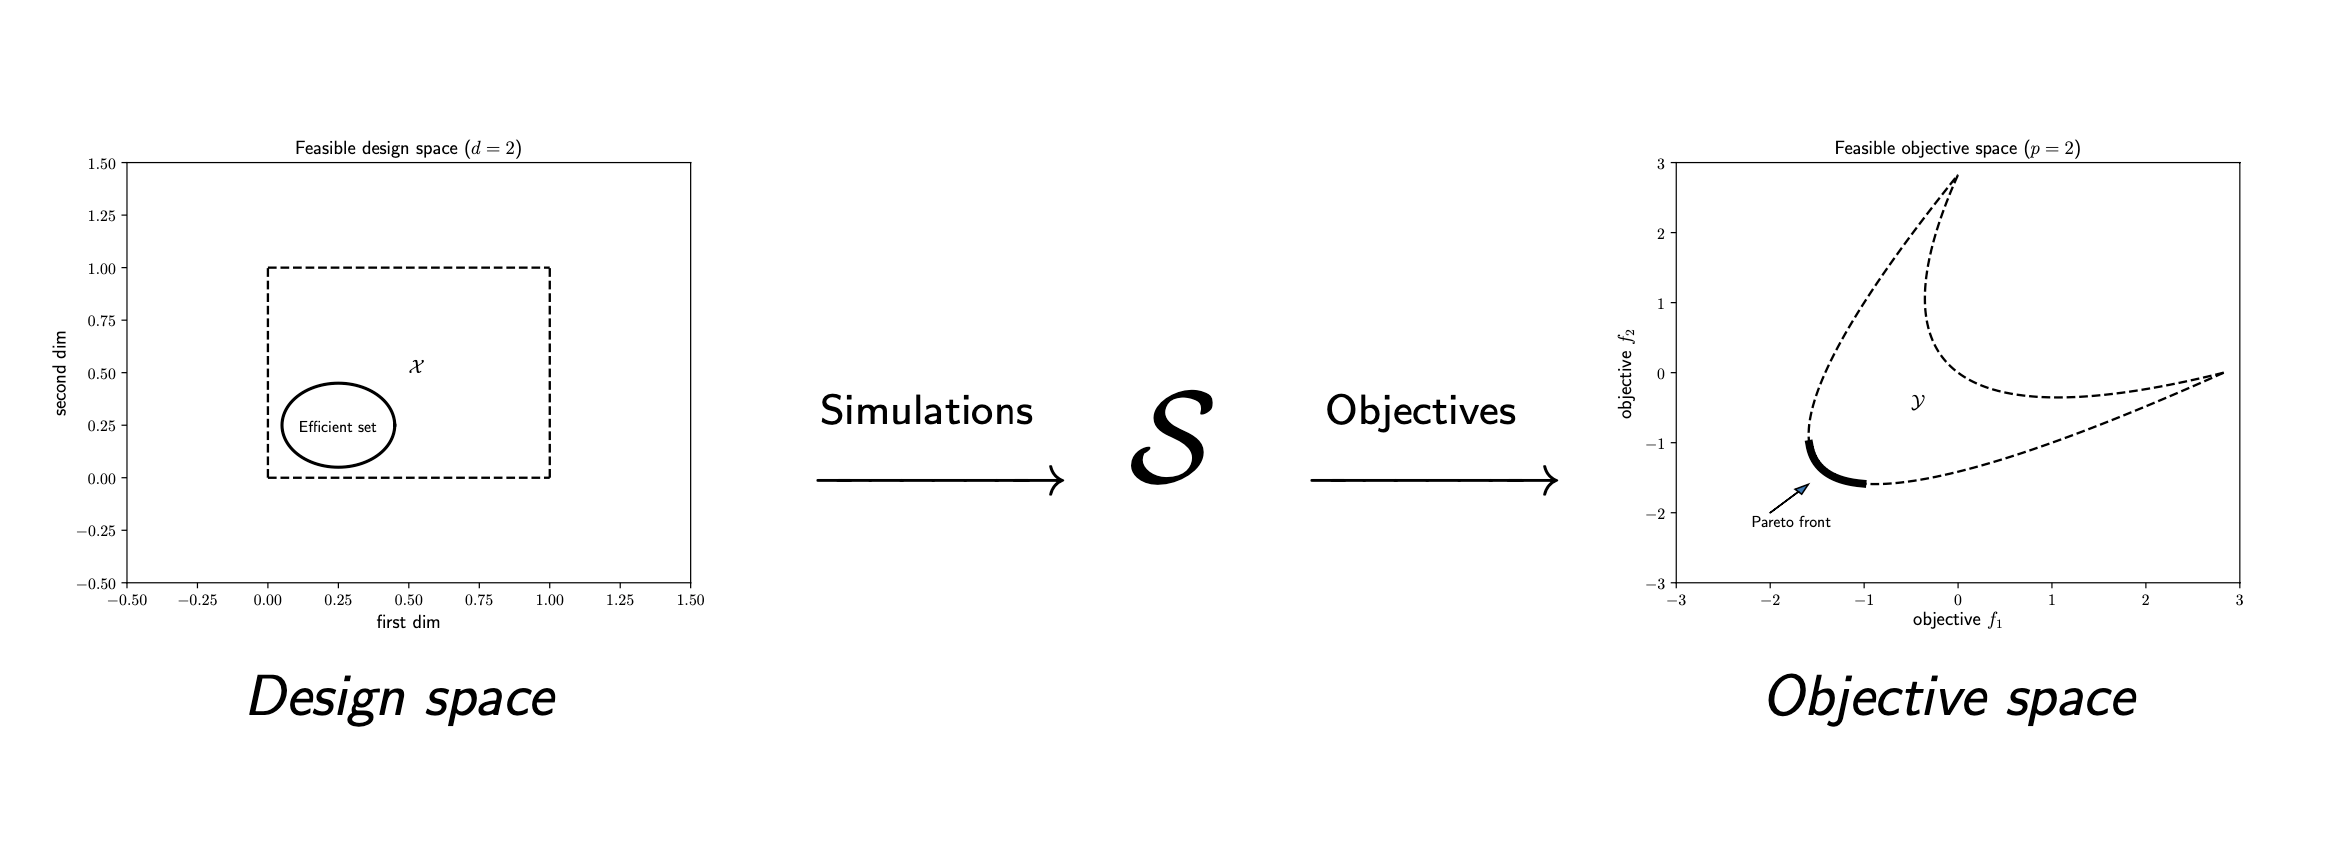
\includegraphics[height=2in]{des-sim-obj-space.png}}
\end{center}
\end{frame}

\begin{frame}\frametitle{Simulation Structure}
{\Large
$$
f_i(x) = {\color{blue}h_i(x, {\color{red}S(x)} )}
\qquad i = 1, \ldots, o
$$
}
\begin{columns}
\begin{column}{0.5\textwidth}
\pause
\textbf{Sum-of-squares structure:}

\medskip

{\large
$$
{\color{blue} h_i(x, S(x)) = \sum_{j \in N_i} \big({\color{red}S_j(x)}\big)^2}
$$

where each ${\color{blue} N_1, \ldots, N_o}$ is an index set.
}

\bigskip

Increases order of approximation $\Rightarrow$
increases order of convergence

\end{column}
\begin{column}{0.5\textwidth}
\pause
\textbf{Heterogeneous MOOPs:}

{\large
\begin{align*}
{\color{red} h_1(x, S(x)) = S_1(x)}\\
{\color{blue} h_2(x, S(x)) = \|x \|^2}
\end{align*}
}

Use expensive surrogate models for {\color{red} $h_1$} (i.e.,
{\color{red} $S_1$}) but not for {\color{blue} $h_2$}

\end{column}
\end{columns}
\end{frame}

\begin{frame}\frametitle{Example 1: Fayans EDF Model Calibration}
Find params $x \in [0, 1]^{13}$ to fit the Fayans model to data $d_i$:
$$
M\left(\xi_{i};x\right) \approx d_{i} \qquad i=1,\ldots, 198
$$

\medskip

ParMOO simulation:
$$
S_{i}(x) = M\left(\xi_{i};x\right) - d_{i},
\qquad i=1,\ldots, 198;
$$

\medskip

\begin{columns}
\begin{column}{0.65\textwidth}
Min SOS across 3 observable classes
\end{column}
\begin{column}{0.35\textwidth}
$$
{\color{blue}F_t = \sum_{i=1}^{m_t}\big({\color{red}S_{t,i}(x)}\big)^2}
$$
\end{column}
\end{columns}

\end{frame}

\begin{frame}\frametitle{Example 2: Material Manufacturing with ParMOO}
Choose optimal settings for material manufacturing in a
continuous flow reactor (CFR)

\bigskip

We know how to make a desired material, need to produce at scale:

\begin{enumerate}
\item {\color{green} \bf Maximize the product} (battery electrolyte: TFML)
\item Can increase temperature to {\bf \color{red} reduce reaction time}
\item Too much heat activates a side reaction; need to
{\bf \color{blue} minimize unwanted byproduct}
\end{enumerate}

\bigskip

{\color{green} \bf Product} and {\color{blue} \bf byproduct} are the result
of expensive experiment,

{\bf \color{red} reaction time} is a controllable input

\end{frame}

\begin{frame}
\begin{center}

\includegraphics[width=0.3\textwidth]{logo-parmoo.png}

\bigskip

{\large
E-mail: {\tt tchang@anl.gov}\\
E-mail: {\tt parmoo@mcs.anl.gov}\\
\bigskip
ParMOO is under review with JOSS\\
\bigskip
GitHub: {\tt github.com/parmoo/parmoo}\\
Docs: {\tt parmoo.readthedocs.io}\\
PyPI: {\tt pip install parmoo}\\
Conda Forge: {\tt conda install --channel=conda-forge parmoo}}\\
\bigskip
{\small This material is based upon work supported by the U.S. Department of Energy, Office of Science, Office of Advanced Scientific Computing Research, SciDAC program under contract number DE-AC02-06CH11357.}
\end{center}
\end{frame}

\end{document}
